\chapter{引言}
\label{chap:intro}

\section{研究背景}
\label{sec:background}
\subsection{大数据研究背景}
随着互联网的快速发展,互联网上的信息呈现了爆发式的增长,互联网已经成为人们获取信
息的一个主要渠道。举个例子,2011年底,新浪微博注册用户数超过3亿,每日发微博量超
过1亿\cite{weibo-info1},在2012年底用户数更是突破
了5亿\cite{weibo-info2}。到2015年, 将会有近30亿人在使用互联网,产生和共享的数据将
达到8ZB\footnote{1 ZB = $10^{21}$B}\cite{bigdata-info}。随着我们可以获得的数据量
的不断增加,人们的研究工作也受到了新的挑战。传统的数据处理手段正愈发显示出其局限
性,如何有效对海量的数据进行处理,进而挖掘出我们所需要的内容逐渐成为一个重要的问
题。近几年,“大数据”迅速成为计算机科学领域非常受关注研究方向。

Doug Laney在\cite{3V}中,提出了“大数据”的3个特点:容量(volume)、速度
(velocity)和多样性(variety)。容量是指数据的存储量非常大,通常在TB,甚至PB级别;
速度是指数据的产生速度很快;多样性是指产生的数据多种多样,没有一个固定的类型,大
部分都是以非结构化和半结构化数据的形式存在。这些是我们在面对大数据时所需要解决的
主要问题。

之前数据挖掘方面许多研究,更多地是关注如何在有限数据的情况下尽可能多地提取出准确
的我们关心的信息。由于受到数据量的限制,很多数据中隐藏的模式和信息并不能被有效地
发现。如今,海量的数据使得数据本身不再是我们研究中的瓶颈,我们关注的重点更多的在
于如何从这些有大量重复冗余的数据中找到我们真正关心的那部分信息,将信息提取出来,
组成结构化的信息,用于计算机的后续处理。
\subsection{结构化数据简介}
\label{sec:structuredata1}
从结构上来看,数据可以分为非结构化数据,半结构化数据和结构化数据。结构化数据是指
可通过明确的结构,如表或者树的格式,进行统一表示的数据。关系数据库和定义良好
的XML就是存储结构化数据的两个典型例子。非结构化的数据没有统一的格式,比如各种各样
的文本、图像、声音、视频等。半结构化的数据则有一定的结构,但结构并不固定,有些字
段可能会扩充或者删除。目前人们日常所接触的大部分万维网上的信息,大部分都是通
过HTML文档进行表示的,HTML文档就是一种典型的半结构化数据,不同的文档在结构上可能
有很大的变化。可以看出,非结构化数据和半结构化的数据更适用于人机界面的交互,而结
构化数据则对机器更加友好。为了便于用计算机进行存储和后续处理,在用计算机处理各种
各样的数据的时候,我们常常希望能将其他的非结构化或者半结构化的数据转化成结构化的
数据进行表示。

这篇文章中,我们主要关心的对象是半结构化的HTML文档。为了更好地对HTML文档进行处理,
我们需要将HTML文档中我们关心的信息提取出来,用结构化数据的方式(比如XML)进行存储。
例如,对于我们获得的博客数据,我们主要关心其中的标题,正文和评论的信息,那么可以
建立一个XML文档,其中的字段都是固定的,每个文档对应一个\texttt{document}节
点,\texttt{document}节点下面
有\texttt{author},\texttt{content}和\texttt{comment}三个子节点。我们将每个博客
的HTML中对应部分抽取出来,存储到该XML文档中。如\reffig{intro:fig:blog-to-xml}所示。
\begin{figure}
  \centering
  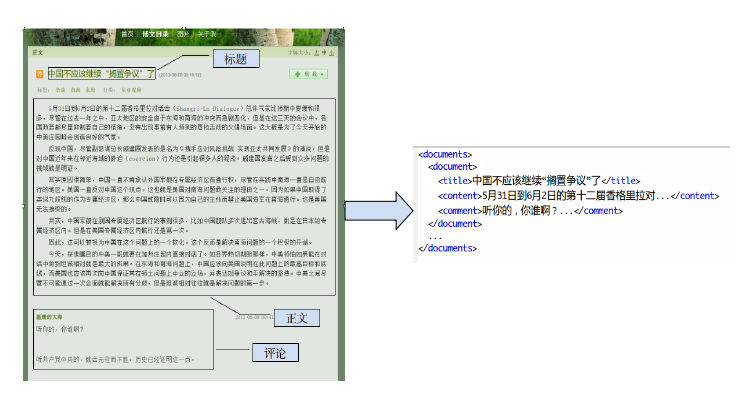
\includegraphics[width=\textwidth]{intro01/blog-to-xml}
  \caption{用XML存储博客的正文,标题和评论}
  \label{intro:fig:blog-to-xml}
\end{figure}

\subsection{HTML文档的模板}
\label{sec:htmltemplateintro}
互联网上有成千上万的HTML文档,对于大部分的网站来说,不可能针对每一个网页单独写一
个静态网页存储到服务器。实际上,我们在互联网上浏览的大部分HTML网页都是通过网站的
后台程序动态生成的,只有极少量的还是通过静态HTML方式进行存储。

在Web开发领域,MVC(Model, View, Controller)模式是目前最流行的开发方法。模型
(Model)是对底层数据和业务的进行的封装;视图(View)负责用户界面的交互,包括给用
户发送信息,接受用户输入等;控制器(Controller)则是系统的控制逻辑,对用户请求进
行处理,用选择合适的视图用于显示模型返回的数据。
如\reffig{intro:fig:mvc}所示\footnote{来
  源:http://en.wikipedia.org/wiki/Model\%E2\%80\%93view\%E2\%80\%93controller}。
目前有很多基于MVC模式的Web开发框架,比如基于Ruby语言的Ruby on Rails,基于Python语
言的Django以及基于Scala语言的Play! Framework等等。这些框架用模型对底层的数据库进
行包装,当用户请求一个HTML页面的时候,控制器负责从数据库中查询相应数据,然后在视
图层选择合适的渲染模板,将对应的数据填充到模板中,从而生成目标HTML文档,将其返回
给用户。\reffig{intro:fig:django}是一个简单的用Django开发网站时视图层的模板示例,
其中\texttt{news.title}和\texttt{news.content}是从数据库中得到的查询结果。
\begin{figure}
  \begin{minipage}[t]{0.5\linewidth}
  \centering
  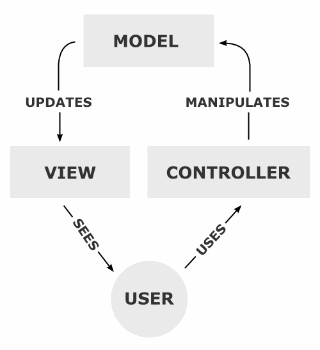
\includegraphics[width=0.5\textwidth]{intro01/MVC-Process}
  \caption{MVC模式}
  \label{intro:fig:mvc}
  \end{minipage}
  \begin{minipage}[t]{0.5\linewidth}
  \centering
  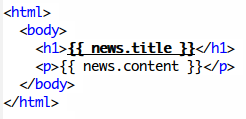
\includegraphics[width=0.6\textwidth]{intro01/django}
  \caption{Django中的HTML模板示例}
  \label{intro:fig:django}
  \end{minipage}
\end{figure}

我们注意到,大部分HTML网页都是通过这种查询底层数据库得到相应数据,然后使用模板进
行渲染的方法生成的。对于大量的从同一个模板生成的网页来说,“模板”就是这些网页
的“公共部分”。实际上,模板的定义要比这里所说的网页的“公共部分”要复杂一些,许
多Web开发框架的模板引擎都支持一些简单的控制结构(如if,for等),如果生成模板的时
候使用了这些控制逻辑,对应的模板也会比较复杂,如\reffig{intro:fig:django-hard}所
示。我们在~\ref{chap:template}中将会给出一个较为严格的定义,这里我们先使用这种直
观的定义便于理解。如果我们能够从大量的由同一个模板生成的网页中将它们的模板抽取出
来,那么我们就可以用抽取出来的模板对其他的由同一个模板生成的网页进行内容的抽取。
简单来说,有了网页的模板以后,每个网页中非“模板”的部分即可以认为是通过查询后台
数据库得到的数据动态生成的,而这些数据正是我们所需要提取出来的。
\begin{figure}
  \centering
  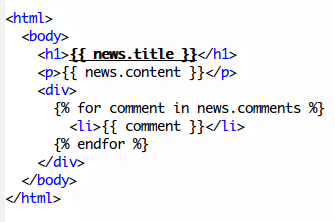
\includegraphics[width=0.5\textwidth]{intro01/django-hard}
  \caption{使用了for的Django模板示例}
  \label{intro:fig:django-hard}
\end{figure}
\section{主要内容与相关工作}
\subsection{主要内容}
\label{sec:mainwork}
本文的主要工作是从已经抓取的大量的网页数据中,自动地对其中的网页进行聚类,得到不
同的类别。对于其中的每一类,将其中可能的模板抽取出来,然后再利用这些模板去抽取新
抓取的网页。由于我们的数据量比较大,因此需要设计一些高效的算法进行抽取;同时,海
量数据也提供了较多的冗余性,使得其中一些隐藏的模式和信息可以更好地被挖掘出来,得
到比较好的实验结果。

互联网上有大量的网站,每个网站的网页都可能采用不同的模板生成。实际上,即使对于同
一个网站,也可能有多个不同的模板。因此,先对这些数据进行聚类是非常必要的,可以尽
早分开相互之间有很大差异的模板所生成的网页。参考~\ref{sec:htmltemplateintro}所述
的网站后台利用模板生成网页过程,我们认为由相同的模板生成的网页,其相似程度主要体
现在仅由HTML标签本身所组成的网页的结构上。我们称这个相似度为网页的结构相似度。与
之类似,HTML文档中所包含的除标签本身以外的内容信息的相似度我们称之为内容相似度。
由于HTML文档中的内容主要来源于后台数据库中查询得到的结果,而数据库中存储的数据本
身没有很大的联系,因此同一模板生成的网页不一定有很高的内容相似度。考虑到这一点,
我们将主要考察HTML文档之间的结构相似度。

在模板提取方面,参考网页后台模板的生成,我们决定主要考虑网页结构上的模板,即由
HTML的标签组成的模板,不考虑HTML文档所包含的内容的相似度。
\subsection{相关工作}
\label{sec:relatedwork}
我们采用基于网页结构相似度的方法进行聚类,
\section{本章总结}
\label{sec:summaryintro}


%%% Local Variables: 
%%% mode: latex
%%% TeX-master: "../main"
%%% End: 

